
\begin{correction}    \;
\begin{enumerate}
%------------------------------
\item \textbf{R\'esolution de $\mathbf{4\sin^2{(x)}-(2+2\sqrt{3})\sin{(x)}+\sqrt{3}\leq 0     }$:}\\
\noindent On pose $X=\sin{(x)}$ et on doit donc r\'esoudre $4X^2-(2+2\sqrt{3})X+\sqrt{3}\leq 0$. Le calcul du discriminant donne $\Delta=(2\sqrt{3}-2)^2$ et on obtient ainsi comme solutions $\ddp\frac{\sqrt{3}}{2}$ et $\ddp\demi$. 
Ainsi :
$$4X^2-(2+2\sqrt{3})X+\sqrt{3}\leq 0 \Leftrightarrow \ddp\demi\leq X\leq \ddp\frac{\sqrt{3}}{2}.$$ 
Comme $X=\sin{(x)}$, on obtient au final que: 
$$4\sin^2{(x)}-(2+2\sqrt{3})\sin{(x)}+\sqrt{3}\leq 0\Leftrightarrow  \ddp\demi\leq \sin{(x)}\leq \ddp\frac{\sqrt{3}}{2}.$$
\begin{minipage}[c]{0.45\textwidth}
La r\'esolution sur le cercle trigonom\'etrique donne
%$$\fbox{$\mathcal{S}_{\R}=\left\lbrace \ddp\frac{\pi}{6}+2k\pi\leq x\leq \ddp\frac{\pi}{3}+2k\pi,\ k\in\Z \right\rbrace\cup\left\lbrace  \ddp\frac{2\pi}{3}+2k\pi\leq x\leq \ddp\frac{5\pi}{6}+2k\pi,\ k\in\Z  \right\rbrace$.}$$
$$\fbox{$\mathcal{S}_{\R}= \ddp \mathop{\bigcup}\limits_{k\in \Z}  \left( \left[ \ddp\frac{\pi}{6}+2k\pi , \ddp\frac{\pi}{3}+2k\pi \right] \cup \left[  \ddp\frac{2\pi}{3}+2k\pi , \ddp\frac{5\pi}{6}+2k\pi\right] \right)$.}$$
\end{minipage}
%\quad \begin{minipage}[c]{0.45\textwidth}
\begin{center}
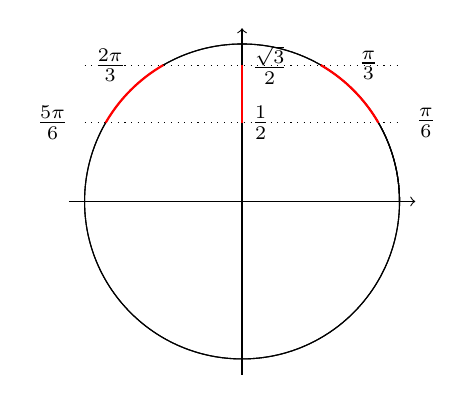
\begin{tikzpicture}[scale=2]
%Axes
\draw [->] (-1.1,0) -- (1.1,0);
\draw [->] (0,-1.1) -- (0,1.1);
%Cercle
\draw (0,0) circle (1);
%Intervalles axes
\draw [red,{[-]}, thick] (0,0.5) -- (0,0.866) ;
%Traits
\draw [dotted] (-1,0.5) -- (1,0.5) ;
\draw [dotted] (-1,0.866) -- (1,0.866) ;
%Points
\draw (0,0.866) node[right] {$\ddp \frac{\sqrt{3}}{2}$};
\draw (0,0.5) node[right] {$\ddp \frac{1}{2}$};
\draw (1,0) arc (0:-210:1) node[left] {$\ddp  \frac{5\pi}{6} \quad $} ;
\draw (1,0) arc (0:30:1) node[right] {$\quad \ddp \frac{\pi}{6}$} ;
\draw (1,0) arc (0:60:1) node[right] {$\quad \ddp \frac{\pi}{3}$} ;
\draw (1,0) arc (0:120:1) node[left] {$\ddp \frac{2\pi}{3}\quad $} ;
%Intervalles cercle
\draw [red, {[-]}, thick] (0.866,0.5) arc (30:60:1) ;
\draw [red, {[-]}, thick] (-0.866,0.5) arc (150:120:1) ;
\end{tikzpicture}
\end{center}
%\end{minipage}
%------------------------------
\item \textbf{R\'esolution de $\mathbf{\tan^2{(x)}-1<0    }$:}\\
\noindent On a: $\tan^2{x}-1<0 \Leftrightarrow -1<\tan{(x)}<1$. La r\'esolution graphique sur le cercle trigonom\'etrique (\`a faire) donne
$$\fbox{$\mathcal{S}_{\R}= \mathop{\bigcup}\limits_{k\in \Z}  \left] -\ddp\frac{\pi}{4}+k\pi , \ddp\frac{\pi}{4}+k\pi \right[$}.$$
%------------------------------
\item \textbf{R\'esolution de $\mathbf{2\cos^2{(3x)}-3\cos{(3x)}+1\leq 0    }$:}\\
\noindent On pose $X=\cos{(3x)}$ et on doit donc r\'esoudre $2X^2-3X+1\leq 0$. 
Le calcul du discriminant donne que les solutions sont $\ddp\demi$ et 1. 
Ainsi $2X^2-3X+1\leq 0 \Leftrightarrow \ddp\demi\leq X\leq 1$. Comme $X=\cos{(3x)}$, on obtient que: $$2\cos^2{(3x)}-3\cos{(3x)}+1\leq 0\Leftrightarrow  \ddp\demi\leq \cos{(3x)}\leq 1.$$ 
\begin{minipage}[c]{0.45\textwidth}
La r\'esolution sur le cercle trigonom\'etrique donne :
$$\ddp\demi\leq \cos{(3x)}\leq 1 \Leftrightarrow \exists k \in \Z, -\ddp\frac{\pi}{3}+2k\pi\leq x\leq \ddp\frac{\pi}{3}+2k\pi.$$
\end{minipage}
\quad \begin{minipage}[c]{0.45\textwidth}
\begin{center}
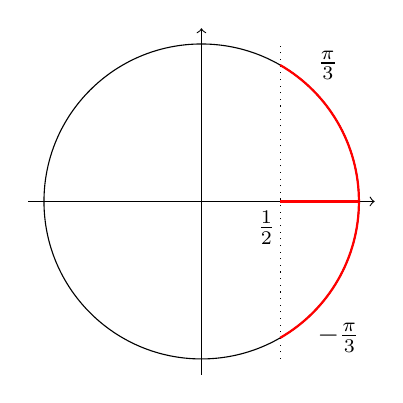
\begin{tikzpicture}[scale=2]
%Axes
\draw [->] (-1.1,0) -- (1.1,0);
\draw [->] (0,-1.1) -- (0,1.1);
%Cercle
\draw (0,0) circle (1);
%Intervalles axes
\draw [red,{]-}, thick] (0.5,0) -- (1,0) ;
%Traits
\draw [dotted] (0.5,-1) -- (0.5,1) ;
%Points
\draw (0.5,0) node[left, below] {$\ddp \frac{1}{2} \quad$};
\draw (1,0) arc (0:-60:1) node[right] {$\quad \ddp - \frac{\pi}{3} $} ;
\draw (1,0) arc (0:60:1) node[right] {$\quad \ddp \frac{\pi}{3}$} ;
%Intervalles cercle
\draw [red, {-[}, thick] (1,0) arc (0:60:1) ;
\draw [red, {-[}, thick] (1,0) arc (0:-60:1) ;
\end{tikzpicture}
\end{center}
\end{minipage}\\
\begin{minipage}[c]{0.45\textwidth}
On obtient donc :
$$\fbox{$\mathcal{S}_{\R}= \ddp \mathop{\bigcup}\limits_{k\in \Z} \left[ -\ddp\frac{\pi}{9}+\ddp\frac{2k\pi}{3}, \ddp\frac{\pi}{9}+\ddp\frac{2k\pi}{3} \right[$}.$$
\end{minipage}
\quad \begin{minipage}[c]{0.45\textwidth}
\begin{center}
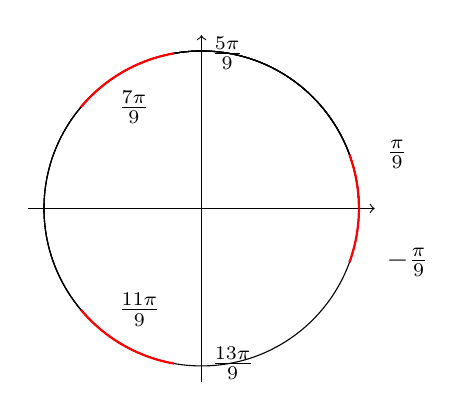
\begin{tikzpicture}[scale=2]
%Axes
\draw [->] (-1.1,0) -- (1.1,0);
\draw [->] (0,-1.1) -- (0,1.1);
%Cercle
\draw (0,0) circle (1);
%Points
\draw (1,0) arc (0:-20:1) node[right] {$\quad \ddp - \frac{\pi}{9} $} ;
\draw (1,0) arc (0:20:1) node[right] {$\quad \ddp \frac{\pi}{9}$} ;
\draw (1,0) arc (0:100:1) node[right] {$\quad \ddp \frac{5\pi}{9} $} ;
\draw (1,0) arc (0:140:1) node[right] {$\quad \ddp \frac{7\pi}{9}$} ;
\draw (1,0) arc (0:220:1) node[right] {$\quad \ddp \frac{11\pi}{9} $} ;
\draw (1,0) arc (0:260:1) node[right] {$\quad \ddp \frac{13\pi}{9}$} ;
%Intervalles cercle
\draw [red, {-]}, thick] (1,0) arc (0:-20:1) ;
\draw [red, {-]}, thick] (1,0) arc (0:20:1) ;
\draw [red, {[-]}, thick] (-0.174,0.985) arc (100:140:1) ;
\draw [red, {[-]}, thick] (-0.766,-0.643) arc (220:260:1) ;
\end{tikzpicture}
\end{center}
\end{minipage}
%------------------------------
\item \textbf{R\'esolution de $\mathbf{\tan^2{(x)}-(\sqrt{3}-1)\tan{(x)}-\sqrt{3}<0    }$:}\\
\noindent On pose $X=\tan{(x)}$ et on doit donc r\'esoudre $X^2-(\sqrt{3}-1)X-\sqrt{3}<0$. Le discriminant vaut $\Delta=(1+\sqrt{3})^2$ et ainsi les solutions sont $-1$ et $\sqrt{3}$. On obtient donc :
$$X^2-(\sqrt{3}-1)X-\sqrt{3}<0 \Leftrightarrow -1<X<\sqrt{3}.$$ 
Comme $X=\tan{(x)}$, on obtient que: 
$$\tan^2{(x)}-(\sqrt{3}-1)\tan{(x)}-\sqrt{3}<0 \Leftrightarrow -1<\tan{(x)}<\sqrt{3}.$$ 
La r\'esolution par le cercle trigonom\'etrique (\`a faire) donne
$$\fbox{$\mathcal{S}_{\R}=\ddp \mathop{\bigcup}\limits_{k\in \Z}  \left] -\ddp\frac{\pi}{4}+k\pi,  \ddp\frac{\pi}{3}+k\pi\right[$}.$$
%------------------------------
\item \textbf{R\'esolution de $\mathbf{\ddp\frac{1}{4}\leq \sin^2{(x)}\leq \ddp\demi   }$:}\\
\noindent On pose $X=\sin{(x)}$ et on doit r\'esoudre $\ddp\frac{1}{4}\leq X^2\leq \ddp\demi$ ce qui est \'equivalent \`{a} $X^2- \ddp\demi\leq 0$ et $\ddp\frac{1}{4}- X^2\leq 0$. Comme 
$X^2- \ddp\demi\leq 0\Leftrightarrow -\ddp\frac{1}{\sqrt{2}}\leq X\leq \ddp\frac{1}{\sqrt{2}}$ et que $\ddp\frac{1}{4}- X^2\leq 0 \Leftrightarrow X\geq \ddp\demi\ \hbox{ou}\ X\leq -\ddp\demi$, on obtient que
$$ \ddp\frac{1}{4}\leq X^2\leq \ddp\demi \Leftrightarrow X\in\left\lbrack -\ddp\frac{1}{\sqrt{2}}, -\ddp\frac{1}{2}\right\rbrack\cup \left\lbrack \ddp\frac{1}{2}, \ddp\frac{1}{\sqrt{2}}\right\rbrack\Leftrightarrow \sin{(x)}\in\left\lbrack -\ddp\frac{1}{\sqrt{2}}, -\ddp\frac{1}{2}\right\rbrack\cup \left\lbrack \ddp\frac{1}{2}, \ddp\frac{1}{\sqrt{2}}\right\rbrack.$$ 
La r\'esolution sur le cercle trigonom\'etrique (\`a faire) donne 
$$\fbox{$\mathcal{S}= \ddp \mathop{\bigcup}\limits_{k\in \Z} \left[ -\ddp\frac{5\pi}{6}+2k\pi, -\ddp\frac{3\pi}{4}+2k\pi \right] \cup \left[ -\ddp\frac{\pi}{4}+2k\pi, -\ddp\frac{\pi}{6}+2k\pi \right] \cup \left[ \ddp\frac{\pi}{6}+2k\pi,  \ddp\frac{\pi}{4}+2k\pi \right] \cup\left[ \ddp\frac{3\pi}{4}+2k\pi, \ddp\frac{5\pi}{6}+2k\pi\right]$}.$$
%------------------------------
\item \textbf{R\'esolution de $\mathbf{\cos{(x)}-\sin{(x)}\geq \ddp\frac{\sqrt{6}}{2}   }$:}\\
\noindent On reconna\^{i}t la forme $a\cos{(x)}+b\sin{(x)}$ et on obtient donc
$$\cos{(x)}-\sin{(x)}\geq \ddp\frac{\sqrt{6}}{2} \Leftrightarrow \sqrt{2}\left( \ddp\frac{1}{\sqrt{2}} \cos{(x)}-\ddp\frac{1}{\sqrt{2}}\sin{(x)}  \right)\geq \ddp\frac{\sqrt{6}}{2}\Leftrightarrow \cos{\left(x  +\ddp\frac{\pi}{4} \right)}\geq \ddp\frac{\sqrt{3}}{2}.$$
On a ainsi obtenu une in\'egalit\'e fondamentale de type $\cos{(X)}\geq \ddp\frac{\sqrt{3}}{2}$ (avec ici $X=x+\ddp\frac{\pi}{4}$) et on r\'esout donc cela graphiquement sur le cercle trigonom\'etrique (\`a faire). On obtient alors
$$\cos{\left(x  +\ddp\frac{\pi}{4} \right)}\geq \ddp\frac{\sqrt{3}}{2} \Leftrightarrow \exists k\in\Z,\ -\ddp\frac{\pi}{6}+2k\pi\leq x+\ddp\frac{\pi}{4}\leq \ddp\frac{\pi}{6}+2k\pi\Leftrightarrow  \exists k\in\Z,\ -\ddp\frac{5\pi}{12}+2k\pi\leq x\leq -\ddp\frac{\pi}{12}+2k\pi.$$
On obtient donc les solutions suivantes:
$$\fbox{$\mathcal{S}_{\R}= \ddp \mathop{\bigcup}\limits_{k\in \Z} \left[  -\ddp\frac{5\pi}{12}+2k\pi, -\ddp\frac{\pi}{12}+2k\pi \right]$}.$$
%------------------------------
\item \textbf{R\'esolution de $\mathbf{\sin{(x)}-\ddp\frac{1}{\sqrt{3}}\cos{(x)}\leq -1}$:}\\
\noindent On reconna\^{i}t la forme $a\cos{(x)}+b\sin{(x)}$ et on obtient donc
$$\sin{(x)}-\ddp\frac{1}{\sqrt{3}}\cos{(x)}\leq -1 \Leftrightarrow -\ddp\frac{2}{\sqrt{3}}\left( \ddp\demi \cos{(x)}-\ddp\frac{\sqrt{3}}{2}\sin{(x)}  \right)\leq -1\Leftrightarrow \cos{\left(x  +\ddp\frac{\pi}{3} \right)}\geq \ddp\frac{\sqrt{3}}{2}.$$
On a chang\'e le sens de l'in\'egalit\'e car $-\ddp\frac{2}{\sqrt{3}}<0$. On a ainsi obtenu une in\'egalit\'e fondamentale de type $\cos{(X)}\geq \ddp\frac{\sqrt{3}}{2}$ (avec ici $X=x+\ddp\frac{\pi}{3}$) et on r\'esout donc cela graphiquement sur le cercle trigonom\'etrique (\`a faire). On obtient alors
$$\cos{\left(x  +\ddp\frac{\pi}{3} \right)}\geq \ddp\frac{\sqrt{3}}{2} \Leftrightarrow \exists k\in\Z,\ -\ddp\frac{\pi}{6}+2k\pi\leq x+\ddp\frac{\pi}{3}\leq \ddp\frac{\pi}{6}+2k\pi\Leftrightarrow  \exists k\in\Z,\ -\ddp\frac{\pi}{2}+2k\pi\leq x\leq -\ddp\frac{\pi}{6}+2k\pi.$$
On obtient donc les solutions suivantes:
$$\fbox{$\mathcal{S}_{\R}=\ddp \mathop{\bigcup}\limits_{k\in \Z} \left[  -\ddp\frac{\pi}{2}+2k\pi, -\ddp\frac{\pi}{6}+2k\pi \right]$}.$$
%------------------------------
\item \textbf{R\'esolution de $\mathbf{\cos{(x)}+\sin{(x)}-1<0   }$:}\\
\noindent On reconna\^{i}t la forme $a\cos{(x)}+b\sin{(x)}$ et on obtient donc
$$\cos{x}+\sin{x}-1<0 \Leftrightarrow \cos{\left( x-\ddp\frac{\pi}{4} \right)}<\ddp\frac{1}{\sqrt{2}}.$$
La r\'esolution sur le cercle trigonom\'etrique (\`a faire) donne: 
$$\cos{\left( x-\ddp\frac{\pi}{4} \right)}<\ddp\frac{1}{\sqrt{2}} \Leftrightarrow \exists k\in\Z,\ \ddp\frac{\pi}{4}+2k\pi <  x-\ddp\frac{\pi}{4} <\ddp\frac{7\pi}{4}+2k\pi \Leftrightarrow \exists k\in\Z,\ \ddp\frac{\pi}{2}+2k\pi <  x <2\pi+2k\pi .$$
On obtient donc :
$$\fbox{$\mathcal{S}_{\R}=\ddp \mathop{\bigcup}\limits_{k\in \Z} \left]  \ddp\frac{\pi}{2}+2k\pi , 2\pi+2k\pi\right[$}.$$
%------------------------------
\item \textbf{R\'esolution de $\mathbf{ \sqrt{3}\cos{(x)}+\sin{(x)}-\sqrt{2}<0  }$:} M\^{e}me m\'ethode.
$$\sqrt{3}\cos{x}+\sin{x}-\sqrt{2}<0 \Leftrightarrow \sqrt{3}\cos{x}+\sin{x}<\sqrt{2} \Leftrightarrow \cos{\left( x-\ddp\frac{\pi}{6} \right)}<\ddp\frac{1}{\sqrt{2}} $$
On obtient par r\'esolution graphique sur le cercle trigonom\'etrique (\`a faire) :
$$\sqrt{3}\cos{x}+\sin{x}-\sqrt{2}<0 \; \Leftrightarrow  \; \exists k\in\Z,\ \ddp\frac{\pi}{4}+2k\pi <  x-\ddp\frac{\pi}{6} <\ddp\frac{7\pi}{4}+2k\pi.$$ 
Ainsi :
$$\fbox{$\mathcal{S}_{\R}=\ddp \mathop{\bigcup}\limits_{k\in \Z} \left]    \ddp\frac{5\pi}{12}+2k\pi , \ddp\frac{23\pi}{12}+2k\pi\right[$}.$$
\end{enumerate}
\end{correction}